\setlength{\belowdisplayskip}{4pt} \setlength{\belowdisplayshortskip}{4pt}
\setlength{\abovedisplayskip}{4pt} \setlength{\abovedisplayshortskip}{4pt}

We begin with a description of our uncertain multivariate data and the corresponding attribute space, followed by a discussion of trait specification, choice of distance metric, generation of feature level-sets, and finally, generation of feature confidence level-sets.
%
Finally, Figure~\ref{fig:example} provides a notional example of the different steps involved to generate the level-sets and is referenced in Sections~\ref{sec:fls} and~\ref{sec:fcls}.
%

\vspace{-2mm}
\subsection{Uncertain Multivariate Data}
%
\fix{From~\cite{jankowai2020feature}, general multivariate data are a set of scalar, vector, or tensor fields $\{F_1,F_2,...,F_r\}$ in the domain $D \subset \mathbb{R}^{3}$, where $r\in\mathbb{N}$ and $r\geq2$.}
%
%
%From~\cite{jankowai2020feature}, general multivariate data are a set of fields
%\begin{equation}
%\left\{F_{1},F_{2},...,F_{r}\right\}, r\in\mathbb{N}, F_{i}:D_{i} \to R_{i},
%\end{equation}
%where $D_{i} = D \subset \mathbb{R}^{3}$ for all $i$ and $R_{i}$ may be sets of scalar, vectors or tensors, and $r\geq2$.
%
Attribute space $\mathcal{A}$ is the combination of the field values and can further include derived quantities.
%
The dimensionality of $\mathcal{A}$ is the combined dimensionality of all selected field values or derived quantities.
%
Considering this definition of attribute space, multivariate data can be summarized as the mapping
\begin{equation}
f : D \to \mathcal{A} \subset R^{n},
\end{equation}
%
where $n$ is the number of dimensions used to form attribute space. 
%
%For our study, we used a maximum of $n = 3$. 
%
For uncertainty in each dimension $i$ of attribute space, we assumed the normal distribution of values at each grid point in $D$ and represented it using mean ${\mu}_{i}$ and standard deviation ${\sigma}_{i}$. 

\vspace{-2mm}
\subsection{Trait Specification}
Traits can be defined generally as artibrary geometries in attribute space $\mathcal{A}$ whose equivalent counterparts in the spatial domain $D$ are identified as features, i.e., $T\subset\mathcal{A}$.
%
A trait can be of any dimension and structure, including points, intervals, lines, and volumes.
%
%The specification of complex traits in a high-dimensional attribute space is a non-trivial task.
%
For simplicity, we assume a limited definition of a trait $T$ by considering intervals for each dimension $i$ of attribute space $\mathcal{A}$
%
\begin{equation}	
T = \forall{i}\;[L_{i}, U_{i}], \;\;L_{i} \leqslant U_{i}, 
\end{equation}
where $L_{i}$ is the lower bound, and $U_{i}$ is the upper bound of the interval for each dimension.
%
As an example, in a visualization of $\mathcal{A}$ for $n = 2$ using a scatterplot, a trait by our definition would be a rectangular selection.

\vspace{-2mm}
\subsection{Distance Metric}
%
%We assume a non-empty feature for our selection of trait $T$.

The feature and feature confidence level-sets are extracted from distance fields.
%
Our objective is to visualize the feature and feature confidence level-sets via the corresponding zero level-sets~(see Sections~\ref{sec:fls} and~\ref{sec:fcls}, respectively). 
%
To achieve this, we computed distance fields using the Euclidean distance transformation~(EDT) algorithm by Saito et al.~\cite{saito1994new} in the spatial domain directly.
%
\fix{The field derived from the EDT algorithm is computed for each grid point in the spatial domain and encodes the distance from a feature.
%
A distance field computed in the spatial domain allows a domain information-guided selection of small threshold distances, whereas distance fields derived from attribute space can be harder to interpret due to dynamic ranges among attributes.}
%
In ~\cite{jankowai2020feature}, the distance field is computed in attribute space to address empty features.
%
In the event that a trait $T$ results in an empty feature, our choice of distance metric would result in a constant distance field.
%
\begin{figure}[!b]
\vspace{-5mm}
\centering
\begin{subfigure}{0.243\linewidth}
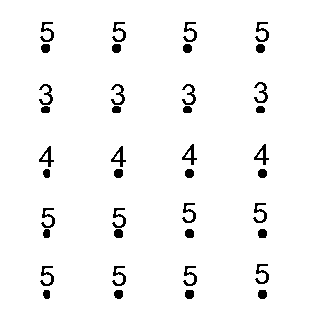
\includegraphics[width=\linewidth]{Images/mu.pdf}
\vspace{-5mm}
\caption{${\mu}$}
\label{fig:mu}
\end{subfigure}
\begin{subfigure}{0.243\linewidth}
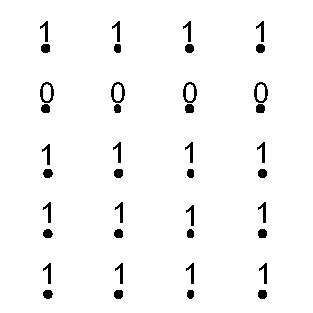
\includegraphics[width=\linewidth]{Images/bvolumeT.pdf}
\vspace{-5mm}
\caption{$bvolume_{T}$}
\label{fig:bvolumeT}
\end{subfigure}
\begin{subfigure}{0.243\linewidth}
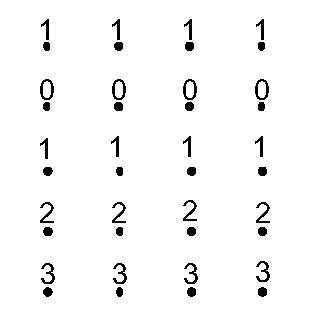
\includegraphics[width=\linewidth]{Images/distanceT.pdf}
\vspace{-5mm}
\caption{$distance_{T}$}
\label{fig:distanceT}
\end{subfigure}
\begin{subfigure}{0.243\linewidth}
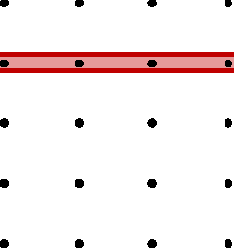
\includegraphics[width=\linewidth]{Images/zlsT.pdf}
\vspace{-5mm}
\caption{$ZLS_{T}$}
\label{fig:zlsT}
\end{subfigure}
\begin{subfigure}{0.243\linewidth}
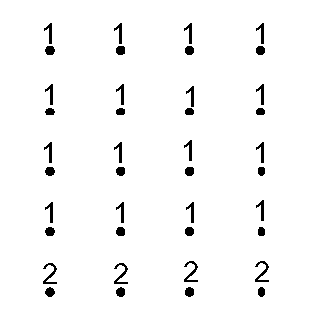
\includegraphics[width=\linewidth]{Images/sigma.pdf}
\vspace{-5mm}
\caption{${\sigma}$}
\label{fig:sigma}
\end{subfigure}
\begin{subfigure}{0.243\linewidth}
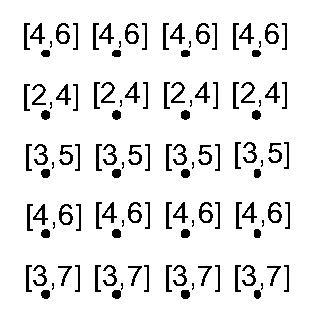
\includegraphics[width=\linewidth]{Images/boundsC.pdf}
\vspace{-5mm}
\caption{$bounds_{C}$}
\label{fig:boundsC}
\end{subfigure}
\begin{subfigure}{0.243\linewidth}
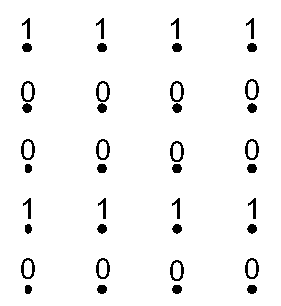
\includegraphics[width=\linewidth]{Images/bvolumeTC.pdf}
\vspace{-5mm}
\caption{$bvolume_{T,C}$}
\label{fig:bvolumeTC}
\end{subfigure}
\begin{subfigure}{0.243\linewidth}
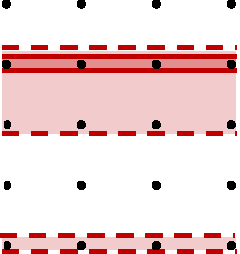
\includegraphics[width=\linewidth]{Images/zlsT_fclsTC.pdf}
\vspace{-5mm}
\caption{{\scriptsize $ZLS_{T}$+$FCLS_{T,C}$}}
\label{fig:fclsTC}
\end{subfigure}
\caption{A notional example showing the steps involved in generating the ``zero'' feature level-set $ZLS_{T}$~(top row) and feature confidence level-set $FCLS_{T,C}$~(bottom row) for an uncertain univariate field represented using ${\mu}$~(a) and ${\sigma}$~(e).
%
For this example, we use trait $T=[2.5, 3.5]$ and confidence $C=68\%$, i.e., $Z=1$.
%
$FCLS_{T,C}$ is computed using the $distance_{T,C}$ (not shown) field.
%
Assuming a unit distance between adjacent grid points,
%
$distance_{T,C}$ would be computed using $bvolume_{T,C}$~(g) as input and would appear equivalent for this example.
%$bvolume_{T,C}$~(g) and $distance_{T,C}$ (not shown) would appear equivalent for this example.
}
\label{fig:example}
\vspace{-5mm}
\end{figure}


\vspace{-2mm}
\subsection{Feature Level-Sets}
\label{sec:fls}
In general, a feature is defined as the pre-image of the trait $T$ in the spatial domain
\begin{equation}
f^{-1}(T) = \left\{ x \in D |\; f(x) \in T \right\}
\end{equation}
%
For our limited definition of a trait $T$ and ${\mu}_{i}$ field of each dimension, a feature is defined as 
\begin{equation}
f^{-1}(T) = \left\{ x \in D |\; \forall i\;{\mu}_{i}(x) \cap [L_{i}, U_{i}] \neq \emptyset\right\}
\end{equation}

\begin{figure*}[!h]
\begin{subfigure}{0.195\linewidth}
\centering
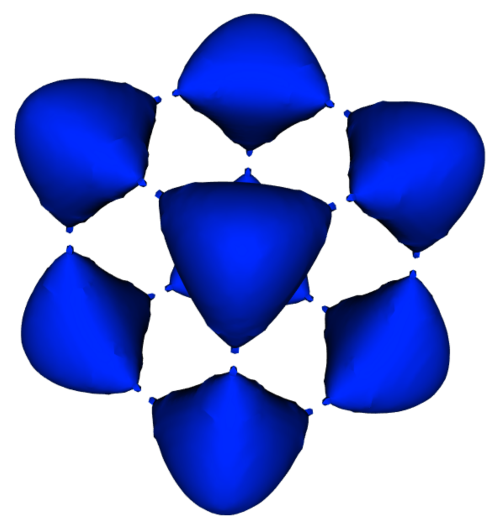
\includegraphics[width=0.8\linewidth]{Images/Tangle/gt.pdf}
\vspace{-2mm}
\caption{Ground truth, $isoval=62$}
\label{fig:tangle_gt}
\end{subfigure}
\begin{subfigure}{0.195\linewidth}
\centering
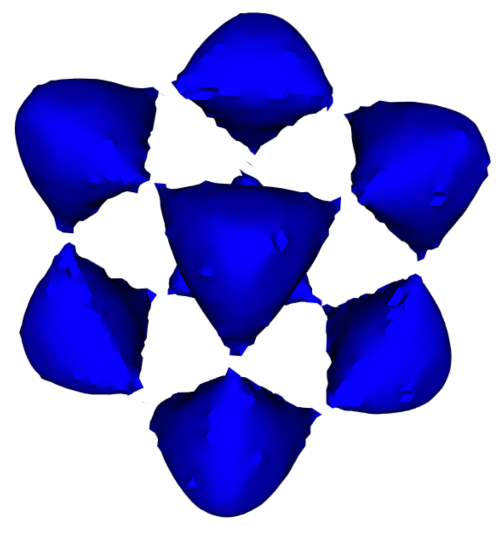
\includegraphics[width=0.8\linewidth]{Images/Tangle/zls.pdf}
\vspace{-2mm}
\caption{$ZLS_{T}$}
\label{fig:tangle_zls}
\end{subfigure}
\begin{subfigure}{0.195\linewidth}
\centering
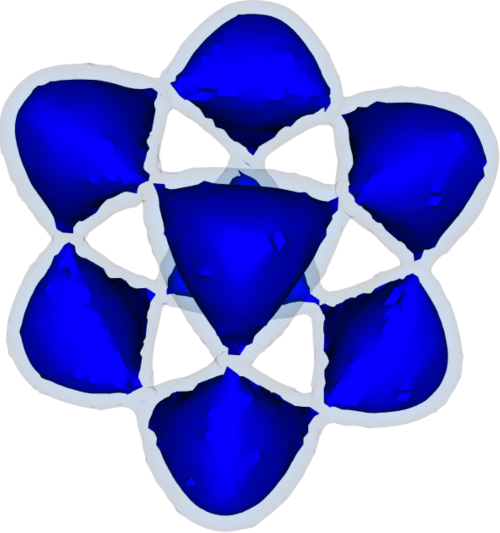
\includegraphics[width=0.8\linewidth]{Images/Tangle/fls.pdf}
\vspace{-2mm}
\caption{$ZLS_{T}$ + $FLS_{T,2}$}
\label{fig:tangle_fls}
\end{subfigure}
\begin{subfigure}{0.195\linewidth}
\centering
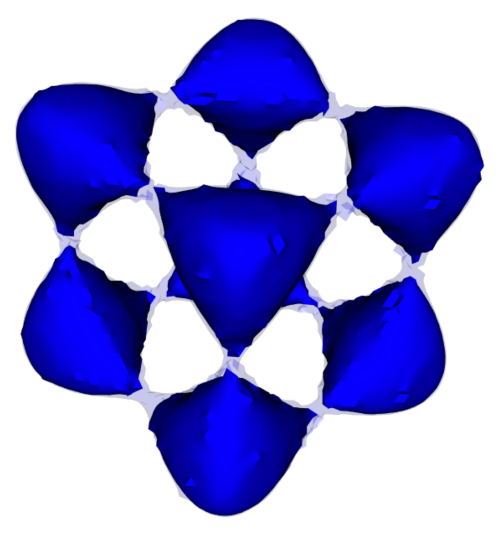
\includegraphics[width=0.8\linewidth]{Images/Tangle/fcls_68.pdf}
\vspace{-2mm}
\caption{$ZLS_{T}$ + $FCLS_{T,68\%}$}
\label{fig:tangle_fcls_68}
\end{subfigure}
\begin{subfigure}{0.195\linewidth}
\centering
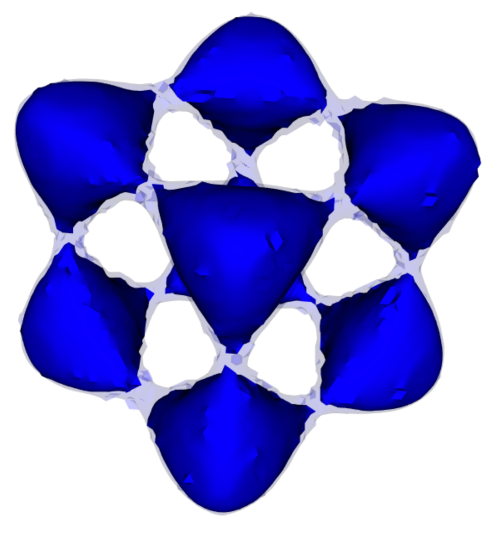
\includegraphics[width=0.8\linewidth]{Images/Tangle/fcls_95.pdf}
\vspace{-2mm}
\caption{$ZLS_{T}$ + $FCLS_{T,95\%}$}
\label{fig:tangle_fcls_95}
\end{subfigure}
\vspace{-2mm}
\caption{Visualization of sensitivity of the tangle function near values that form links between the multiple blobs. We use $T=[0,62]$.}
\vspace{-2mm}
\label{fig:tangle}
\end{figure*}

\begin{figure*}[!h]
\begin{subfigure}{0.20\linewidth}
\centering
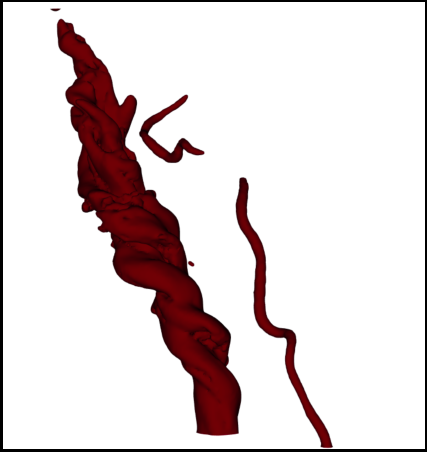
\includegraphics[width=0.9\linewidth]{Images/Tornado/zls.pdf}
\vspace{-1mm}
\caption{$ZLS_{T}$}
\label{fig:tornado_zls}
\end{subfigure}
\begin{subfigure}{0.20\linewidth}
\centering
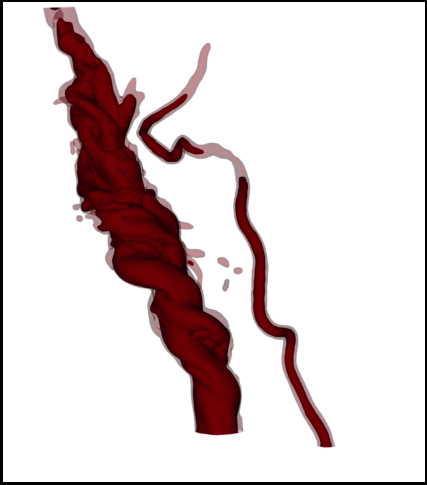
\includegraphics[width=0.9\linewidth]{Images/Tornado/fcls_50.pdf}
\vspace{-1mm}
\caption{+ $FCLS_{T,50\%}$}
\label{fig:tornado_fls}
\end{subfigure}
\begin{subfigure}{0.20\linewidth}
\centering
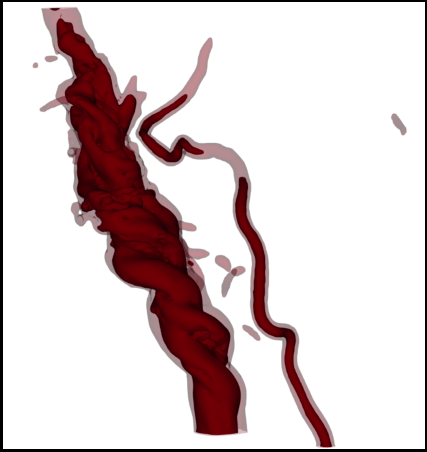
\includegraphics[width=0.9\linewidth]{Images/Tornado/fcls_68.pdf}
\vspace{-1mm}
\caption{+ $FCLS_{T,68\%}$}
\label{fig:tornado_fls}
\end{subfigure}
\begin{subfigure}{0.20\linewidth}
\centering
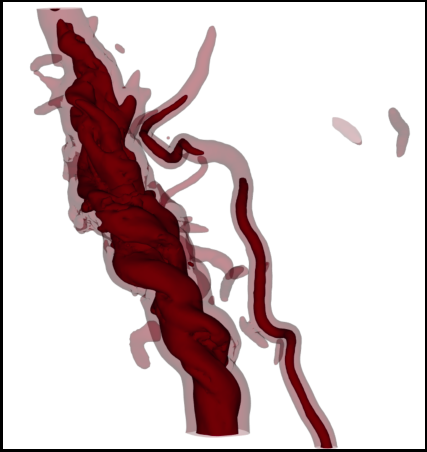
\includegraphics[width=0.9\linewidth]{Images/Tornado/fcls_95.pdf}
\vspace{-1mm}
\caption{+ $FCLS_{T,95\%}$}
\label{fig:tornado_fcls}
\end{subfigure}
\hfill
\begin{subfigure}{0.17\linewidth}
\centering
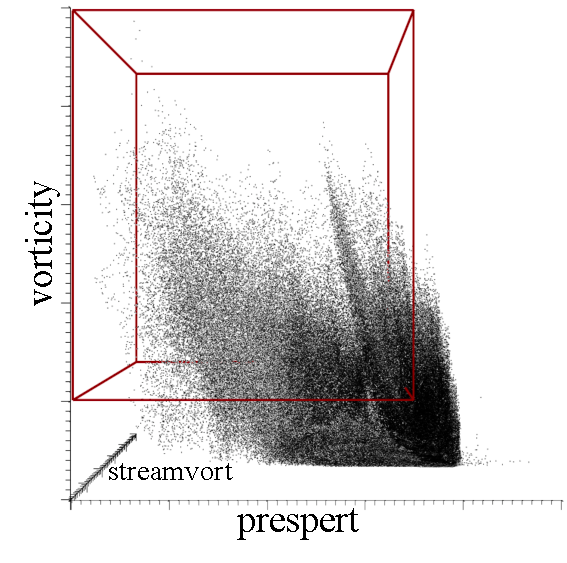
\includegraphics[width=\linewidth]{Images/Tornado/scatterplot3d.pdf}
\vspace{-4mm}
\caption{3D scatterplot of $\mathcal{A}$ and $T$ (red cuboid).} 
\label{fig:tornado_scatterplot}
\end{subfigure}
%\vspace{-2mm}
\caption{Visualization of EF-5 tornado vortices using vorticity, prespert and streamvort attributes. As in Figure~\ref{fig:tangle}, $FCLS_{T,C}$ formed wider envelopes as $C$ increased. Importantly, $FCLS_{T,C}$ visualized vortical structures of interest in the vicinity of the primary tornado vortex.}
%\vspace{-1mm}
\label{fig:tornado}
\end{figure*}



To visualize the feature and its secondary structures, we performed three steps:
%
First, for trait $T$, we computed a binary volume $bvolume_{T}$~(Figure~\ref{fig:bvolumeT}) to represent the absence or existence of the feature at a specific grid point
%
\begin{equation}
  bvolume_{T}(x) = \left \{
  \begin{aligned}
    &0, && \text{if}\; \forall i\; {\mu}_{i}(x) \cap [L_{i}, U_{i}] \neq \emptyset \\
    &1, && \text{otherwise}
  \end{aligned} \right.
\end{equation}
%
Second, we performed EDT using $bvolume_{T}$ as input to produce a distance field $distance_{T}$~(Figure~\ref{fig:distanceT}). 
%
%We used an algorithm proposed by Saito \textit{et al.}~\cite{saito1994new} to perform EDT.
%
As a final step, we computed feature level-set $FLS_{T,K}$ as the level-set of level $K$ of the distance field
%
\begin{equation} 
distance_{T}^{-1}(K) = \left\{ x \in D\; |\; distance_{T}(x) = K\right\}
\end{equation}
%
\fix{Here, the distance at each grid point is the spatial distance from $\forall i\; \mu_{i}(x) \cap [L_{i}, U_{i}] \neq \emptyset$.}
%
For $K = \epsilon$, i.e., a small threshold value near zero, we refer to $FLS_{T,\epsilon}$ as $ZLS_{T}$~(Figure~\ref{fig:zlsT}).
%\fix{Figure~\ref{fig:example} top row illustrates the different steps to generate $FLS_{T,\epsilon}$ or $ZLS_{T}$.}
%
%As the value of $K$ increases, we believe \fix{(instead of saying "we believe", should we refer to ~\cite{jankowai2020feature}, as we did in the Introduction last paragraph?)} its relevance reduces given discernibility concerns and greater distance from the feature in the spatial domain.
%

\vspace{-2mm}
\subsection{Feature Confidence Level-Sets}
\label{sec:fcls}
%
Uncertainty in multivariate data can result in different shapes of $ZLS_{T}$.
%
To assess the uncertainty, we visualized within which envelope the $ZLS_{T}$ will lie for a certain confidence interval $C$.
%
Similar to the steps we used to compute $ZLS_{T}$, to extract feature confidence level-sets $FCLS_{T,C}$, we first identified all the grid points that satisfy the trait $T$ for confidence interval $C$.
%
To achieve this, we used the method by Zehner et al.~\cite{zehner2010visualization}. 
%
We used the $Z$-score, or the number of standard deviations from the mean a value would be, for a given confidence interval $C$, and then, for each dimension $i$, calculated $bounds_{i,C}$~(Figure~\ref{fig:boundsC})
%\fix{(should we replace variable C with variable Z, e.g.,  $bounds_{i,Z}(x)$ and so on, everywhere below? Only a suggestion for improving readability.)}
%\begin{equation}
%bound_{i,lower}(x) = mean_{i}(x) - Z*SD_{i}(x),
%\end{equation}
%\begin{equation}
%bound_{i,upper}(x) = mean_{i}(x) + Z*SD_{i}(x)\\
%\end{equation}
\begin{equation}
%bounds_{i,C}(x) = \forall i \; [bound_{i, lower}(x), bound_{i,upper}(x)]
bounds_{i,C}(x) = \forall i \; [{\mu}_{i}(x) - Z*{\sigma}_{i}(x),~~{\mu}_{i}(x) + Z*{\sigma}_{i}(x)]
\end{equation}
%
Using $bounds_{i,C}$ and $T$, we computed $bvolume_{T,C}$~(Figure~\ref{fig:bvolumeTC})
\begin{equation}
  bvolume_{T,C}(x) = \left \{
  \begin{aligned}
    &0, && \text{if}\; \forall i\; bounds_{i, C}(x) \cap [L_{i}, U_{i}] \neq \emptyset \\
    &1, && \text{otherwise}
  \end{aligned} \right.
\end{equation}
%

Following the extraction of $bvolume_{T,C}$, we performed EDT to compute $distance_{T,C}$.
%
Finally, we extracted the feature confidence level-set $FCLS_{T,C,K}$ as the level-set of level $K$ of the distance field
%
\begin{equation} 
distance_{T,C}^{-1}(K) = \left\{ x \in D\; |\; distance_{T,C}(x) = K\right\}
\end{equation}
\fix{Here, the distance at each grid point is the spatial distance from $\forall i\; bounds_{i,C}(x) \cap [L_{i}, U_{i}] \neq \emptyset$.}
%
Given our objective of visualizing a single level-set extracted from $distance_{T,C}$ with $K = \epsilon$, i.e., a small threshold value near zero, we refer to $FCLS_{T,C,\epsilon}$ as simply $FCLS_{T,C}$~(Figure~\ref{fig:fclsTC}).
%
